% ------------------------------------------------------------------------------
% TYPO3 CMS 7.1 - What's New - Chapter "Backend User Interface" (Pluswerk Version)
%
% @author	Patrick Lobacher <patrick@lobacher.de>
% @license	Creative Commons BY-NC-SA 3.0
% @link		http://typo3.org/download/release-notes/whats-new/
% @language	German
% ------------------------------------------------------------------------------
% LTXE-CHAPTER-UID:		e7264f0e-3f82290d-94c50cda-fb2d8e66
% LTXE-CHAPTER-NAME:	Backend User Interface
% ------------------------------------------------------------------------------

\section{Backend User Interface}
\begin{frame}[fragile]
	\frametitle{Backend User Interface}

	\begin{center}\huge{Kapitel 1:}\end{center}
	\begin{center}\huge{\color{typo3darkgrey}\textbf{Backend User Interface}}\end{center}

\end{frame}

% ------------------------------------------------------------------------------
% LTXE-SLIDE-START
% LTXE-SLIDE-UID:		ce334239-cc6fd2e4-ce4564a6-9061b594
% LTXE-SLIDE-TITLE:		Datepicker
% LTXE-SLIDE-REFERENCE:	Breaking-62925-RemoveExtJsDateTimePicker.rst
% ------------------------------------------------------------------------------

\begin{frame}[fragile]
	\frametitle{Backend User Interface}
	\framesubtitle{Look \& Feel: Neuer Datepicker}

	Der Datepicker im Backend wurde auf Bootstrap umgestellt

	\begin{figure}
		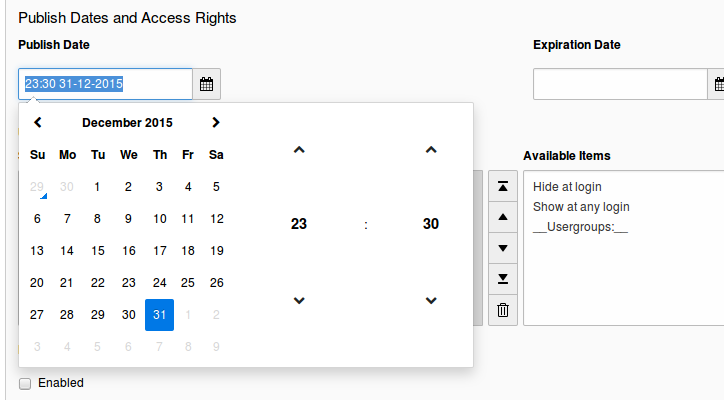
\includegraphics[width=0.90\linewidth]{BackendUserInterface/be-datepicker.png}
	\end{figure}

\end{frame}


% ------------------------------------------------------------------------------
% LTXE-SLIDE-START
% LTXE-SLIDE-UID:		f55164a3-9b110115-60fc5d61-626ab535
% LTXE-SLIDE-TITLE:		Functions Module
% LTXE-SLIDE-REFERENCE:	Breaking-63310-Wizard-Modules-Moved.rst
% ------------------------------------------------------------------------------

\begin{frame}[fragile]
	\frametitle{Backend User Interface}
	\framesubtitle{Look \& Feel: Funktionen Modul}

	"Create Pages" und "Sort Pages" wurde verschoben zu: \texttt{WEB => Functions}\newline
	\smaller (in TYPO3 CMS < 7.1, waren diese unter "\texttt{WEB => Functions => Wizards}" zu finden) 

	\begin{figure}
		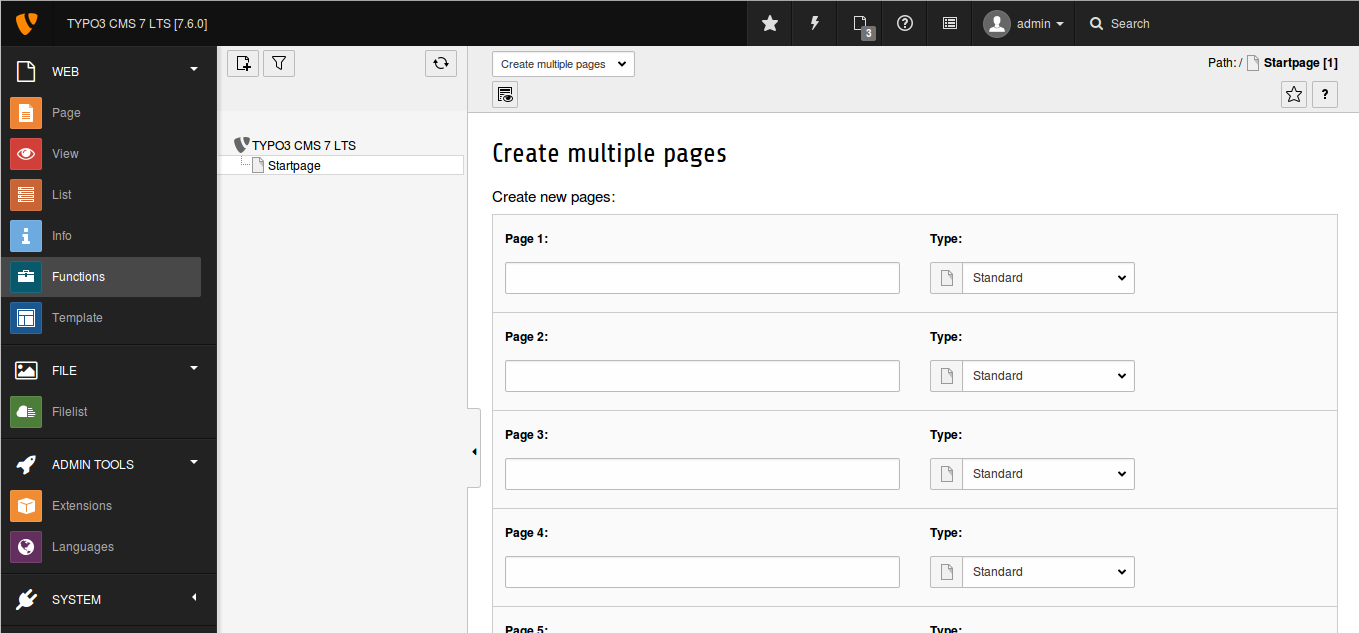
\includegraphics[width=0.80\linewidth]{BackendUserInterface/be-functions.png}
	\end{figure}

\end{frame}


% ------------------------------------------------------------------------------
% LTXE-SLIDE-START
% LTXE-SLIDE-UID:		43bce7ce-da1bc516-dd06ea5c-07d79912
% LTXE-SLIDE-TITLE:		Access Module
% LTXE-SLIDE-REFERENCE:	Feature-15619-LeaveUnchagedInAccessModule.rst
% ------------------------------------------------------------------------------

\begin{frame}[fragile]
	\frametitle{Backend User Interface}
	\framesubtitle{Look \& Feel: Access Modul}

 	Im Modul \texttt{Access} kann man User und/oder Gruppe unverändert (" - leave unchanged -") lassen, wenn man nur die Berechtigungen ändern möchte

	\begin{figure}
		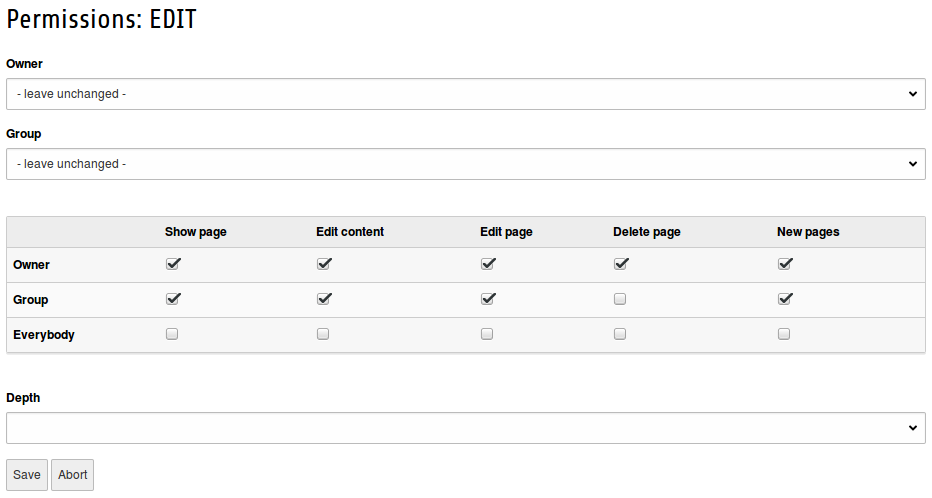
\includegraphics[width=0.75\linewidth]{BackendUserInterface/be-access.png}
	\end{figure}

\end{frame}

% ------------------------------------------------------------------------------
% LTXE-SLIDE-START
% LTXE-SLIDE-UID:		7ec94718-ad988847-632b1e94-e40a667a
% LTXE-SLIDE-TITLE:		Icons im List-Modul
% LTXE-SLIDE-REFERENCE:	Feature-63207-SplitActionButtonsIntoGroups.rst
% ------------------------------------------------------------------------------

\begin{frame}[fragile]
	\frametitle{Backend User Interface}
	\framesubtitle{Look \& Feel: Icons im List-Modul}

	Die Icons im Modul \texttt{Web => List} wurden in zwei Gruppen angeordnet - zuerst die typischen RUD (Read, Update, Delete) Icons und anschließend die weiteren

	\begin{figure}
		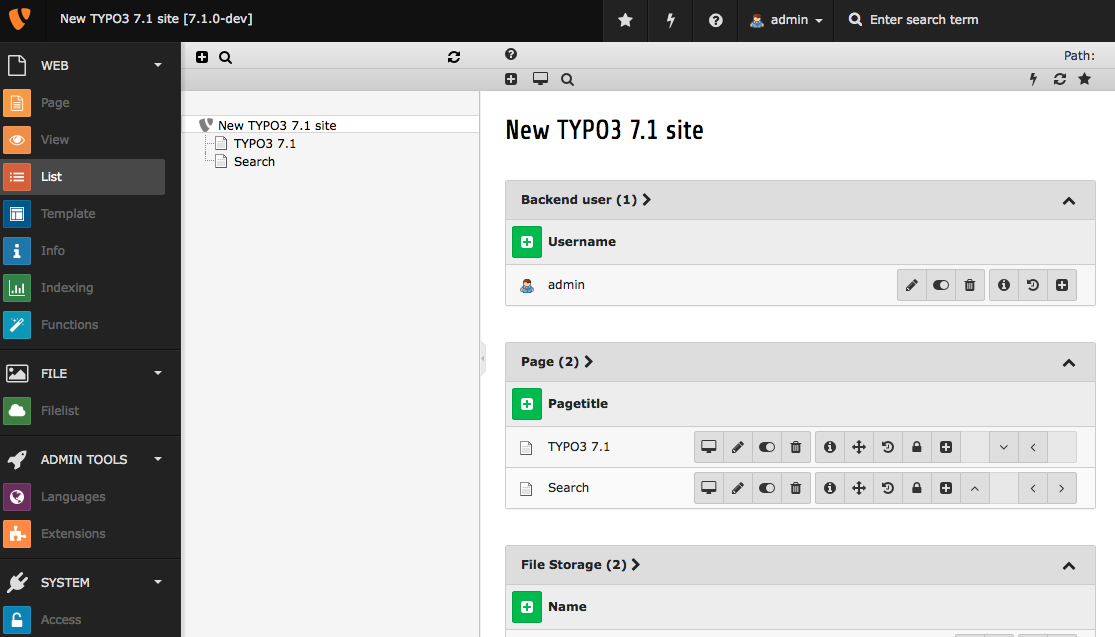
\includegraphics[width=0.75\linewidth]{BackendUserInterface/be-icons.png}
	\end{figure}

\end{frame}
